\documentclass[a4paper]{article}

% Basic packages
\usepackage[fontset=fandol]{ctex}
\usepackage{amsmath, amssymb}
\usepackage{graphicx}
\usepackage[margin=2.4cm]{geometry}
\usepackage[most]{tcolorbox}
\usepackage{etoolbox}
\usepackage{listings}
\usepackage{hyperref}
\usepackage{xurl}
\usepackage{booktabs}
\usepackage{longtable}
\usepackage{tabularx}
\usepackage{array}
\usepackage{subcaption}
\usepackage{float}
\usepackage{enumitem}
\usepackage{tikz}

\hypersetup{
    colorlinks=true,
    linkcolor=blue!50!black,
    urlcolor=blue!60!black,
    citecolor=blue!50!black
}

\newtcolorbox{findingbox}[1]{
    enhanced,
    colback=green!5!white,
    colframe=green!45!black,
    colbacktitle=green!45!black,
    coltitle=white,
    fonttitle=\bfseries,
    title=#1,
    sharp corners
}

\newtcolorbox{evidencebox}[1]{
    enhanced,
    colback=blue!4!white,
    colframe=blue!65!black,
    colbacktitle=blue!65!black,
    coltitle=white,
    fonttitle=\bfseries,
    title=#1,
    sharp corners
}

\newtcolorbox{riskbox}[1]{
    enhanced,
    colback=red!4!white,
    colframe=red!70!black,
    colbacktitle=red!70!black,
    coltitle=white,
    fonttitle=\bfseries,
    title=#1,
    sharp corners
}

\newtcolorbox{methodbox}[1]{
    enhanced,
    colback=yellow!9!white,
    colframe=yellow!60!black,
    colbacktitle=yellow!60!black,
    coltitle=black,
    fonttitle=\bfseries,
    title=#1,
    sharp corners
}

\lstset{
    language=Python,
    basicstyle=\ttfamily\small,
    keywordstyle=\color{blue},
    stringstyle=\color{red!60!black},
    commentstyle=\color{green!50!black},
    breaklines=true,
    frame=single,
    numbers=left,
    numberstyle=\tiny\color{gray},
    captionpos=b,
    extendedchars=false
}

\newcolumntype{Y}{>{\raggedright\arraybackslash}X}
\setlist[itemize]{leftmargin=1.8em}
\setlength{\parskip}{0.5em}

\newcommand{\reporttitle}{Claude Code Hub 半截断流治理升级说明}
\newcommand{\reportsubtitle}{面向运维与产品验收的 Web 可见变化与证据报告}
\newcommand{\reportauthors}{Codex}
\newcommand{\reportdate}{2026-03-25}
\newcommand{\researchquestion}{这次围绕「输出到一半停住」问题的升级，究竟改了哪些模块，以及在当前 Web 控制台里能从哪里观察到这些变化？}
\newcommand{\reportscope}{聚焦 2026-03-25 已部署到生产容器的 Claude Code Hub 版本；覆盖运行时中断归因、Response API 流终止语义、启动迁移自愈，以及它们在现有 Web 控制台中的可观察结果。}
\newcommand{\reportaudience}{Claude Code Hub 的维护者、运维同学与负责验收的产品使用者}
\newcommand{\sourcewindow}{代码与页面证据截止到 2026-03-25 10:10 CST；运行中实例为 127.0.0.1:23000 上的生产容器}
\newcommand{\reportcoverpath}{figures/traffic-logs-502.png}

\begin{document}

\begin{titlepage}
\centering
{\Large 深度研究报告\par}
\vspace{1.0cm}
{\huge\bfseries \reporttitle\par}
\vspace{0.5cm}
{\Large \reportsubtitle\par}
\vspace{0.9cm}
{\large \reportauthors\par}
\vspace{0.2cm}
{\large \reportdate\par}
\vspace{1.0cm}

\includegraphics[width=0.84\textwidth,height=0.42\textheight,keepaspectratio]{\reportcoverpath}\par

\vfill
\begin{tcolorbox}[width=0.94\textwidth, colback=black!2!white, colframe=black!60, sharp corners]
\textbf{核心问题}：\researchquestion\par
\textbf{研究范围}：\reportscope\par
\textbf{目标读者}：\reportaudience\par
\textbf{证据窗口}：\sourcewindow\par
\end{tcolorbox}
\end{titlepage}

\tableofcontents
\newpage

\section{执行摘要}

\begin{findingbox}{结论先行}
这次升级的主体是\textbf{运行时语义修复}，不是一次前端样式改版。最关键的三个升级点分别是：
\begin{itemize}
\item 用统一的 abort diagnosis 取代过去对 \texttt{ResponseAborted} 的粗糙归因，避免把上游半截断流误记成客户端取消。
\item 在 Response API 流已经开始输出后，如果中途失败，Hub 会补发合成的 \texttt{response.failed} 终止事件，而不是静默断掉。
\item 启动迁移加入旧库自愈逻辑，能修补空的 \texttt{drizzle.\_\_drizzle\_migrations} 与缺失列，避免容器重启时再次打出迁移硬失败。
\end{itemize}
\end{findingbox}

从 Web 角度看，\textbf{主要观察入口仍然是控制台的“流量 > 日志”页面}，而不是新增一个专门的“半截断流”页。运维可以在这里过滤 \texttt{502} 失败请求，再结合详情弹窗、导出数据或数据库查询，确认失败是否被归到 \texttt{STREAM\_*} 分类。与此同时，管理后台的登录页和“系统 > 日志”配置页在这次升级后仍能正常访问，说明这次发布没有带来明显的 Web 管理面回归。

\section{研究范围与方法}

\begin{methodbox}{范围假设}
用户没有要求做一份纯技术设计文档，而是明确要求“讲讲现在升级的哪个地方，要有对应的截图”。因此本报告采用如下边界：
\begin{itemize}
\item 重点回答“升级了什么”与“在当前 Web 上如何观察”。
\item 只纳入本次已经部署到生产容器的改动，不扩展到历史所有优化。
\item 报告中的截图全部来自运行中的实例，而不是本地未发布预览页。
\end{itemize}
\end{methodbox}

本报告建立在多模态证据之上，证据类型包括：
\begin{itemize}
\item 代码：运行时归因、流终止与迁移自愈实现。
\item Web 截图：登录页、流量日志页、系统日志配置页。
\item 运维输出：容器健康状态、启动日志、健康检查接口。
\item 结构化数据：\texttt{message\_request} 中 \texttt{CLIENT\_ABORTED} 与 \texttt{STREAM\_*} 错误统计。
\end{itemize}

\begin{evidencebox}{证据强度}
本报告的大部分主张来自一手证据：已部署容器的运行状态、仓库内代码实现、数据库当前统计与本人在生产实例上的截图。唯一的次级来源是已有的内部说明文档，用来帮助组织叙述而非作为核心事实依据。
\end{evidencebox}

\section{升级内容总览}

\begin{table}[H]
\centering
\small
\begin{tabularx}{\textwidth}{p{2.8cm}p{4.2cm}p{3.5cm}Y}
\toprule
升级点 & 核心实现 & 直接证据 & 当前 Web 可见位置 \\
\midrule
中断归因统一化 &
引入 \texttt{diagnoseAbortError}，把 abort 细分为 \texttt{client\_abort}、\texttt{response\_timeout}、\texttt{stream\_idle\_timeout}、\texttt{upstream\_abort} 等 &
\texttt{src/app/v1/\_lib/proxy/errors.ts:764--820} &
最直接体现在“流量 > 日志”的失败解释会更准确，但主表仍主要显示状态码 \\
\addlinespace
Response API 流终止补偿 &
对已开始输出的 Response 流，在异常中断时补合成 \texttt{response.failed} 事件 &
\texttt{src/app/v1/\_lib/proxy/response-handler.ts:197--289} &
主要影响 VS Code / Codex 等 Response 客户端；Web 日志页负责观察落库结果 \\
\addlinespace
迁移启动自愈 &
检测空 journal 的旧库，补缺列并 baseline \texttt{drizzle.\_\_drizzle\_migrations} &
\texttt{src/lib/migrate.ts:32--48, 179--365} &
没有新增 UI；效果是发布后后台可正常启动，管理面不再被迁移失败拖垮 \\
\bottomrule
\end{tabularx}
\caption{本次升级的三个核心模块与其 Web 观察点}
\end{table}

\section{Web 端具体体现}

\subsection{登录面稳定，说明本次发布不是 UI 改版}

图 \ref{fig:login-page} 展示的是这次发布后实际运行中的登录页。视觉结构、入口文案与表单交互都保持稳定，没有新增字段、开关或入口。这一点很重要：它说明本轮升级的主轴并不是“换一套管理后台界面”，而是修复流式中断与启动可靠性。

\begin{figure}[H]
\centering
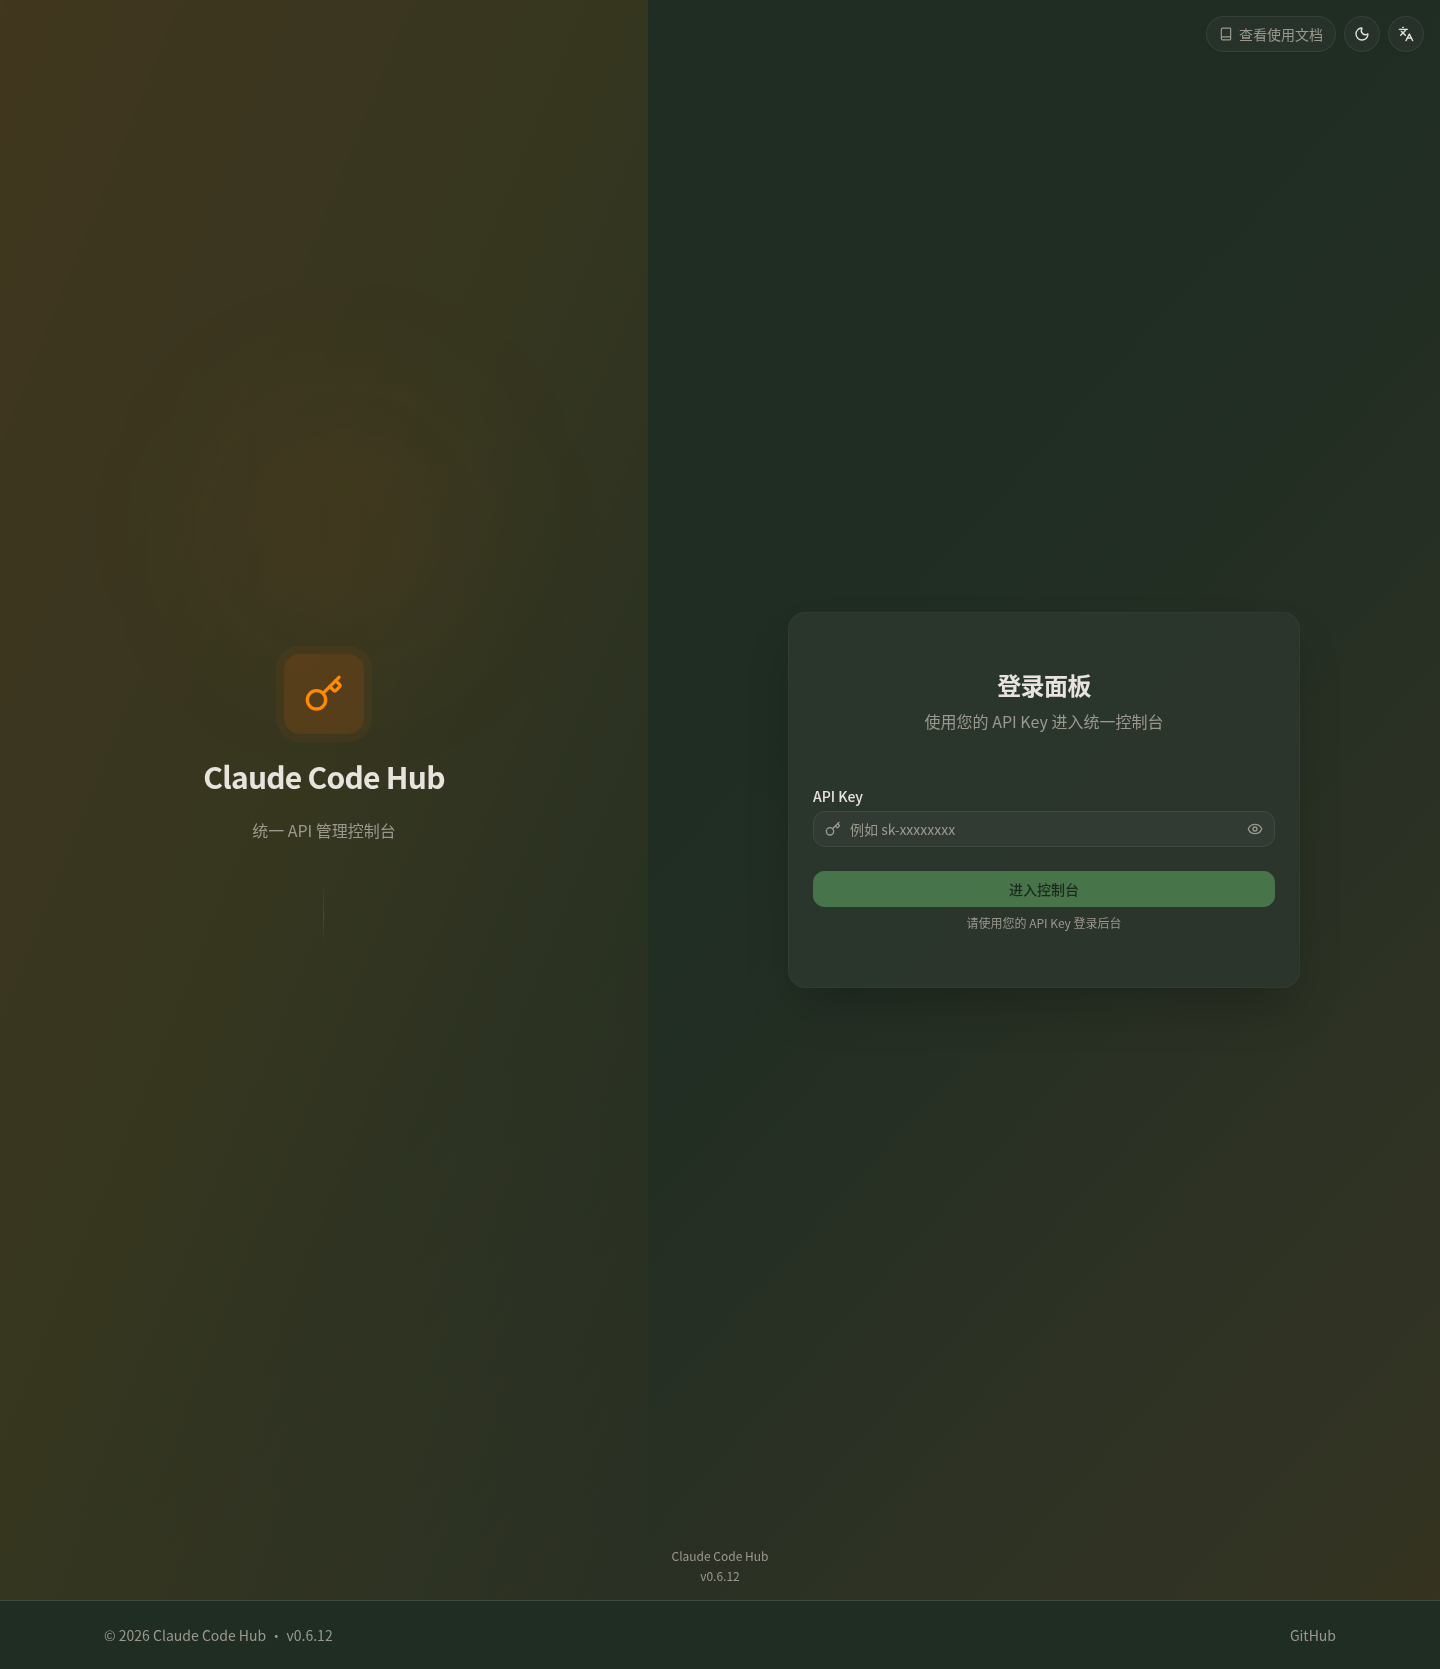
\includegraphics[width=0.84\textwidth]{figures/login-page.png}
\caption{部署后登录页截图。来源：2026-03-25 从运行中的实例 \url{http://127.0.0.1:23000/zh-CN/login} 截取。}
\label{fig:login-page}
\end{figure}

\begin{evidencebox}{如何解读这张图}
这张图本身不代表“升级发生在登录页”，而是用于证明：发布后的基础管理入口仍然健康可用，没有因为运行时修复而引入明显的 Web 回归。
\end{evidencebox}

\subsection{“流量 > 日志”是本次升级最主要的 Web 观察入口}

图 \ref{fig:traffic-logs} 展示了控制台 \texttt{/zh-CN/console/traffic/logs?statusCode=502} 页面。主表中可以直接看到多条红色 \texttt{502} 失败请求记录，这正是本次“半截断流治理”最重要的运营观察面。

\begin{figure}[H]
\centering
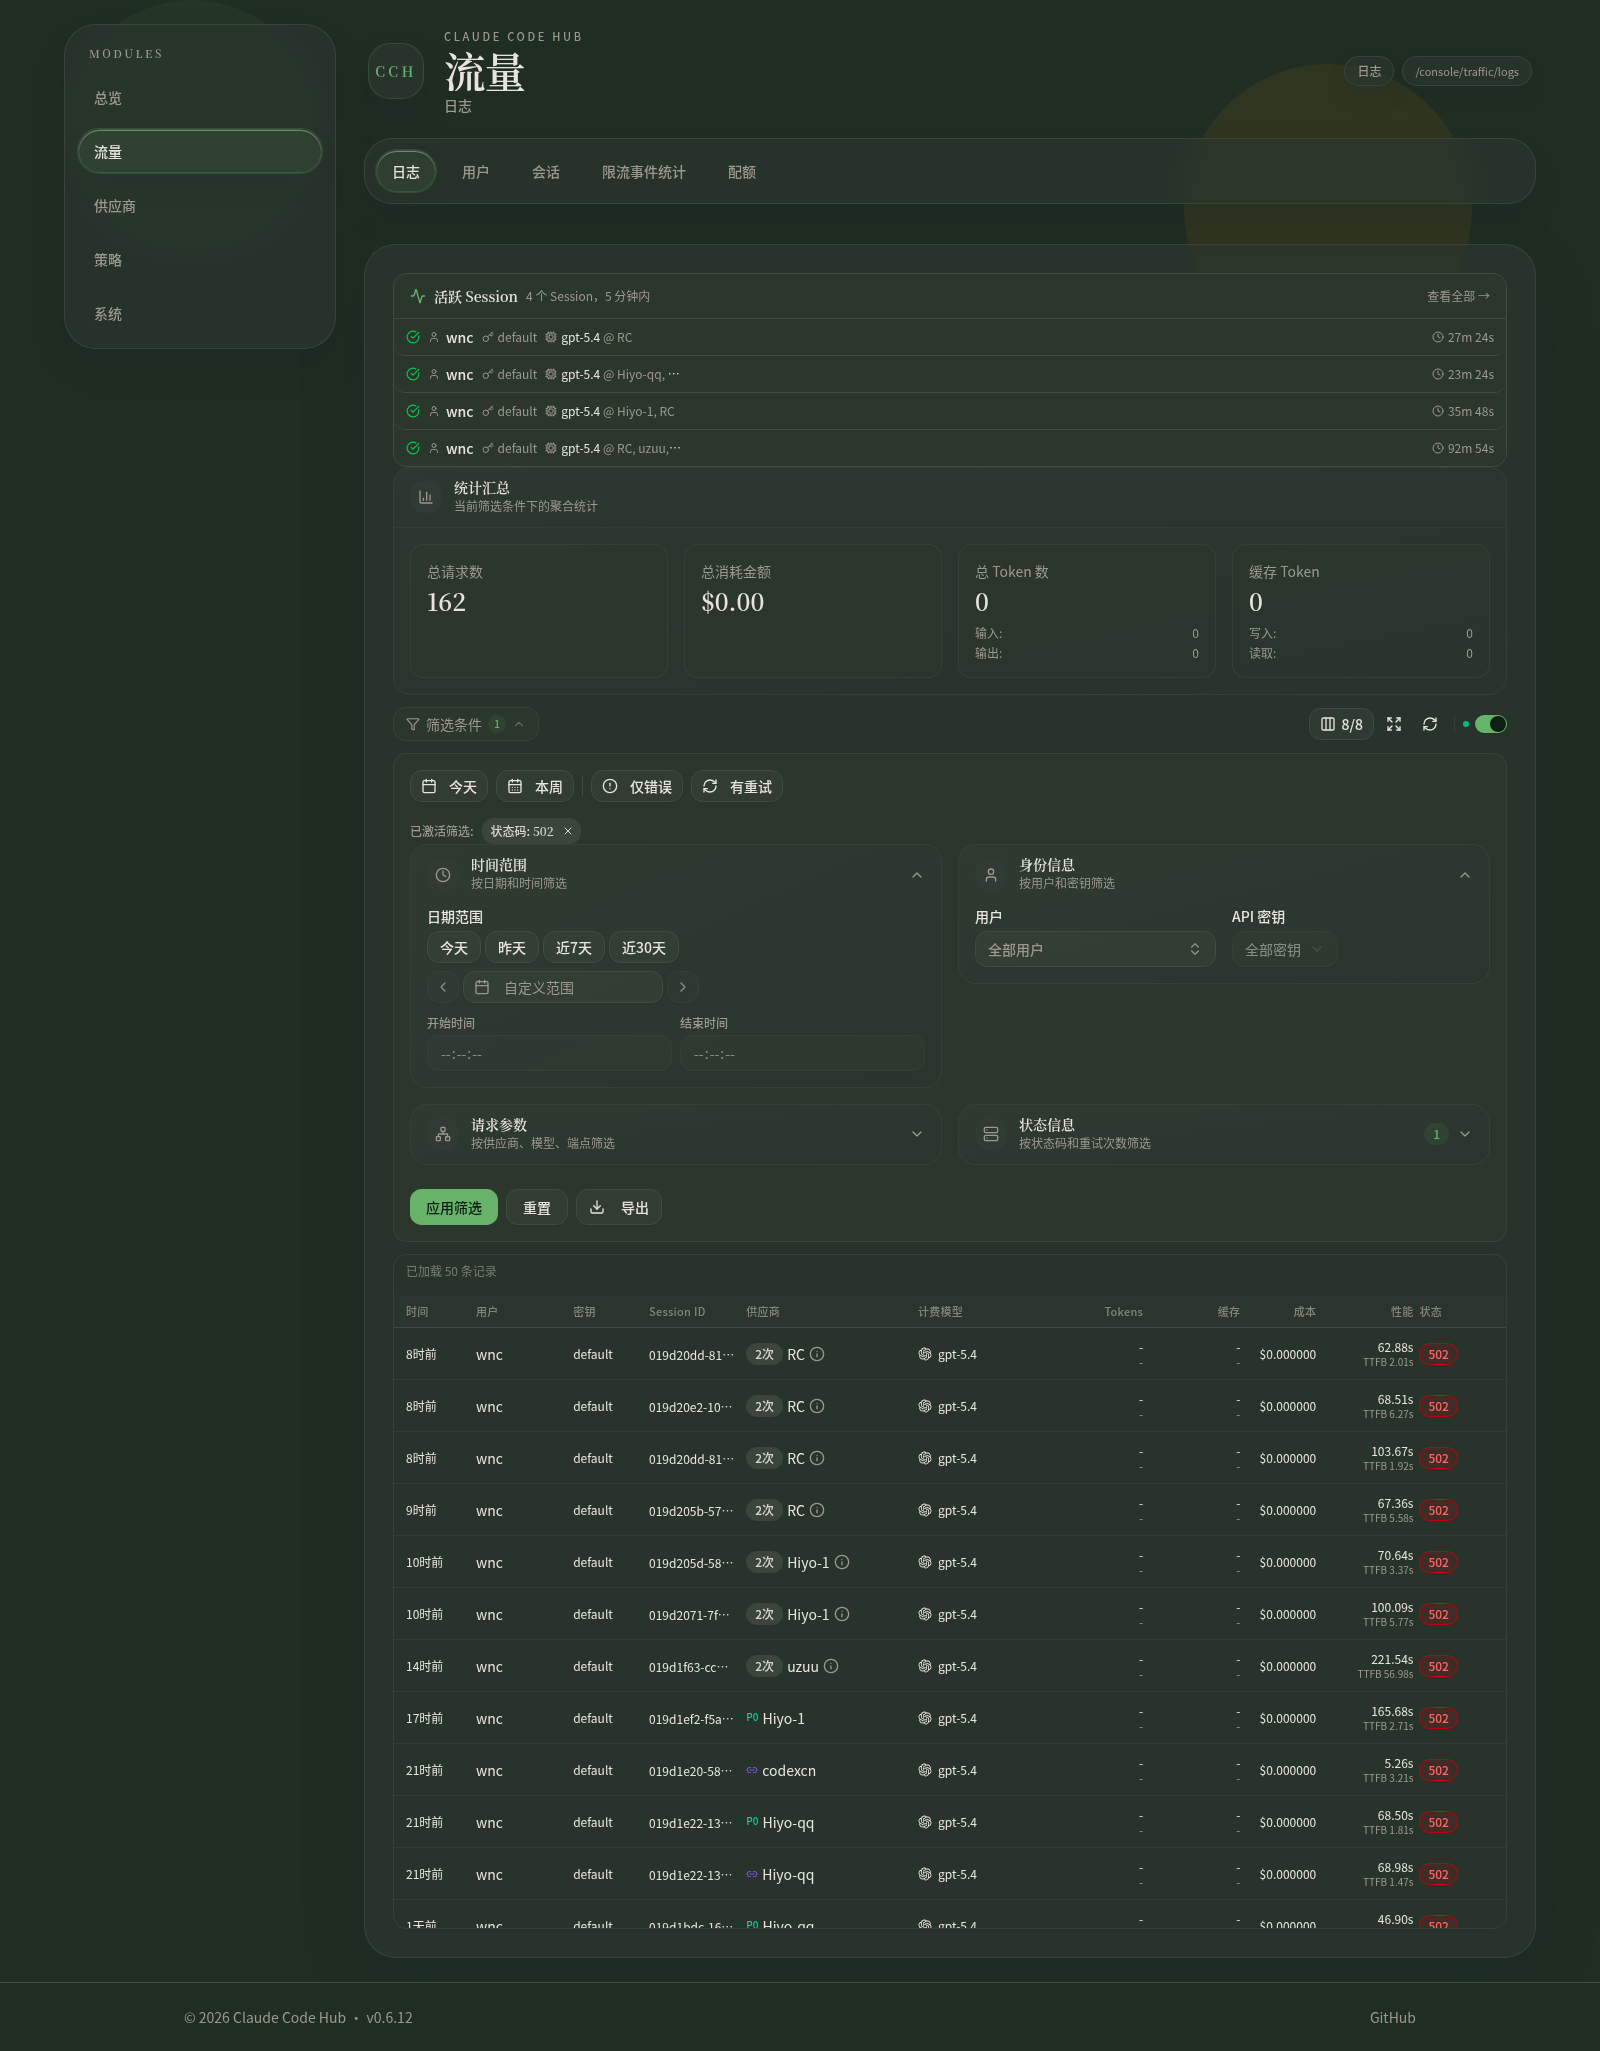
\includegraphics[width=\textwidth]{figures/traffic-logs-502.png}
\caption{控制台“流量 > 日志”页面，已按 \texttt{statusCode=502} 过滤。来源：2026-03-25 从运行中的实例 \url{http://127.0.0.1:23000/zh-CN/console/traffic/logs?statusCode=502} 截取。}
\label{fig:traffic-logs}
\end{figure}

这里需要特别说明一个容易误解的点：\textbf{这次升级让失败“归因更准”，但主表的第一层视觉仍然主要显示 HTTP 状态码，不会自动变成满屏的 \texttt{STREAM\_*} 标签。} 换句话说，Web 主表的“可见变化”更像是“哪些失败值得你点进去看”，而不是新增了一列完全不同的 UI 元素。

当前数据库快照表明，系统已经把一部分失败请求稳定落成 \texttt{STREAM\_*} 语义，而不是全部都塞进 \texttt{CLIENT\_ABORTED}：

\begin{table}[H]
\centering
\small
\begin{tabular}{lrr}
\toprule
\texttt{error\_message} & \texttt{status\_code} & 计数 \\
\midrule
\texttt{CLIENT\_ABORTED} & 499 & 1255 \\
\texttt{STREAM\_UPSTREAM\_ABORTED} & 502 & 23 \\
\texttt{STREAM\_PROCESSING\_ERROR} & 502 & 7 \\
\texttt{STREAM\_IDLE\_TIMEOUT} & 502 & 3 \\
\bottomrule
\end{tabular}
\caption{截至 2026-03-25 的 \texttt{message\_request} 关键错误分类快照}
\end{table}

\begin{findingbox}{对运维的实际意义}
这张表说明现在至少有三类“中途断流”失败已经能在后端被稳定拆分出来。运维在 Web 上最合理的操作顺序是：
\begin{itemize}
\item 先在“流量 > 日志”中过滤 \texttt{502}
\item 再打开失败详情，查看错误信息与逻辑链路
\item 如需更细粒度核对，可结合导出或数据库查询确认是否落成了 \texttt{STREAM\_*}
\end{itemize}
\end{findingbox}

\subsection{“系统 > 日志”页保持可用，但它是配置面，不是实时日志查看器}

图 \ref{fig:system-logs-page} 是系统模块下的“日志”页面。它本质上是日志级别配置页，而不是实时日志滚动面板。因此，这次升级在这里的意义不在于出现了新的按钮，而在于：\textbf{升级后的后台仍能正常打开这类管理配置页，说明迁移和容器启动已恢复稳定。}

\begin{figure}[H]
\centering
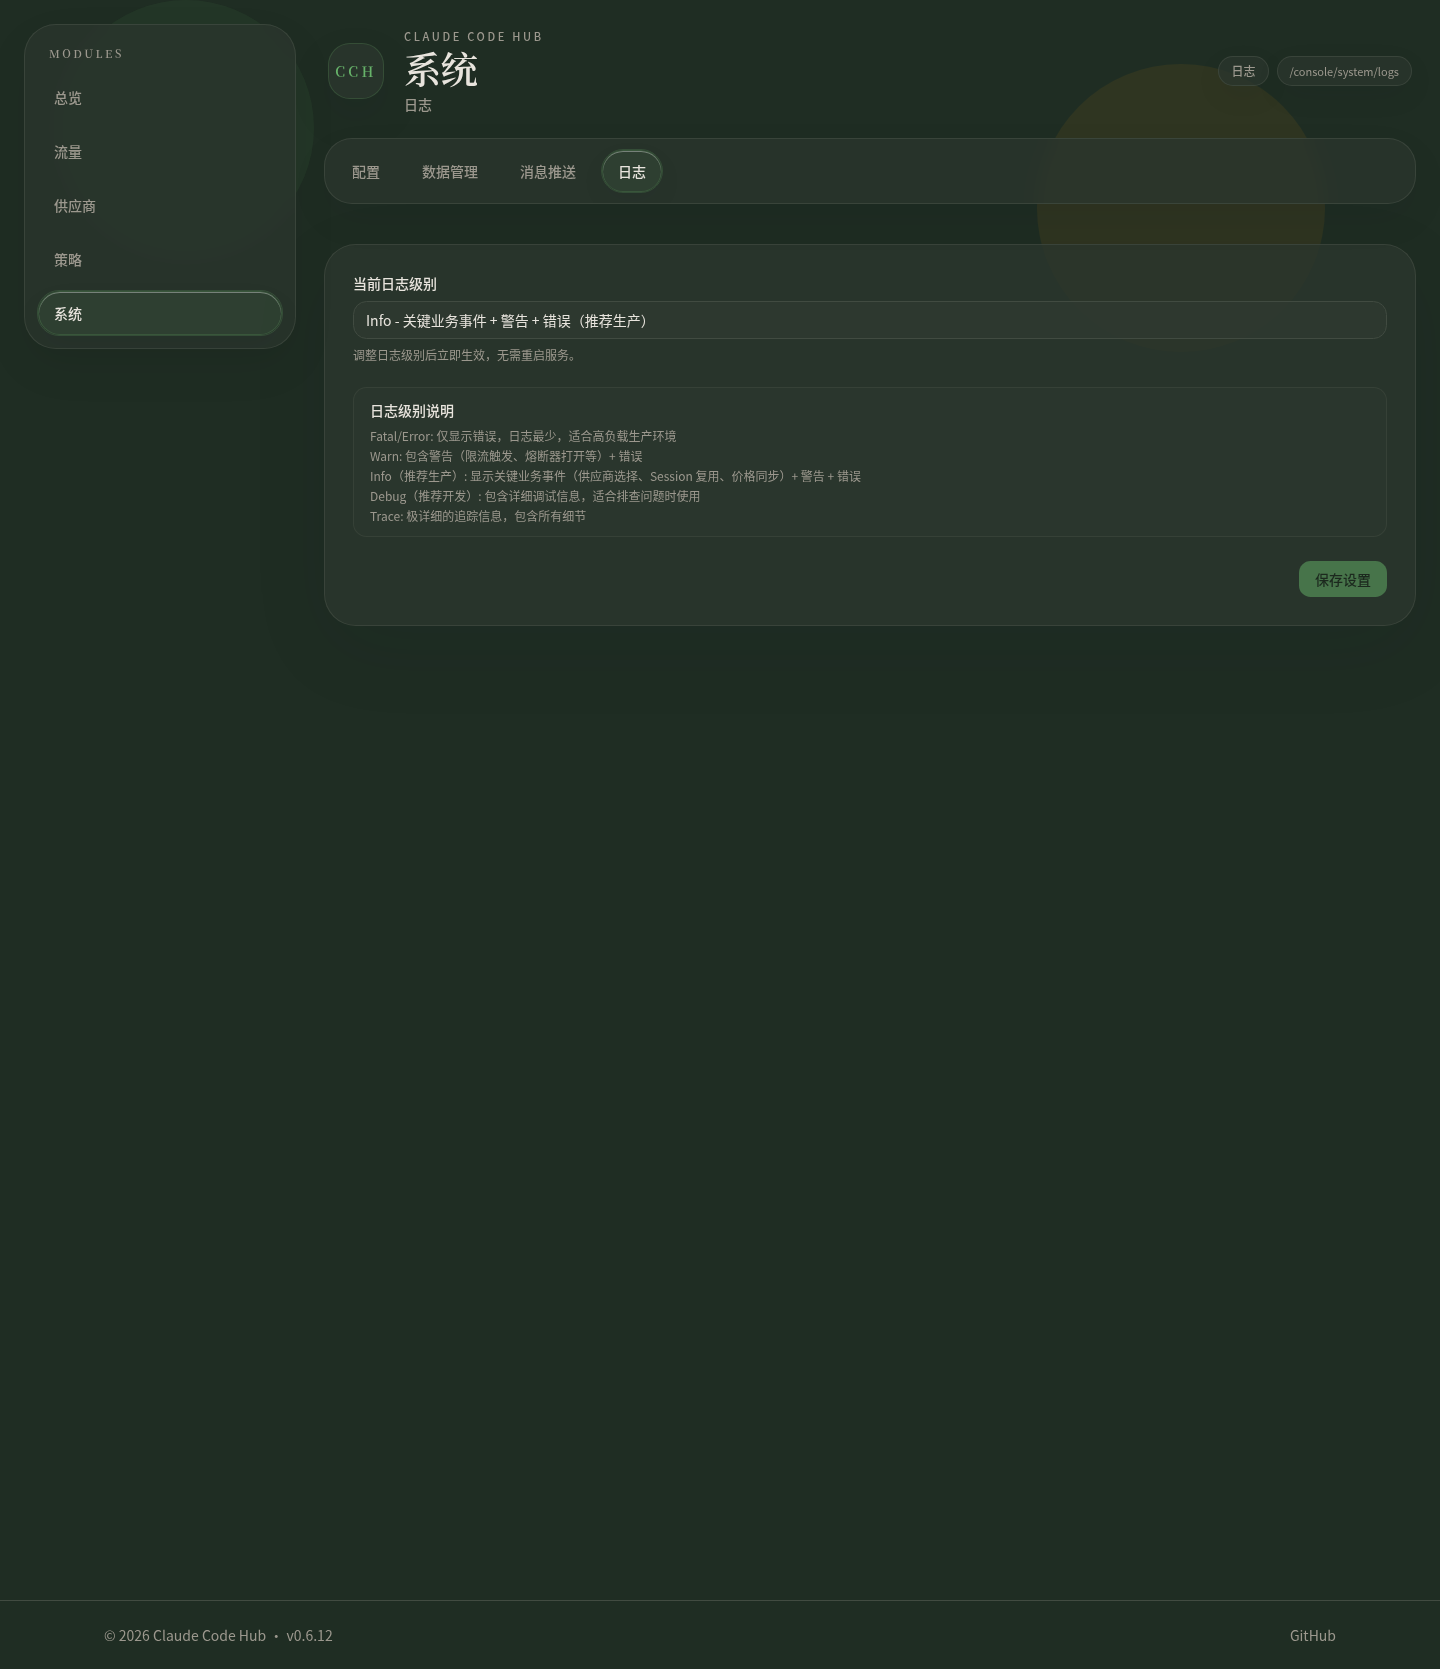
\includegraphics[width=\textwidth]{figures/system-logs-page.png}
\caption{系统模块下的日志配置页面。来源：2026-03-25 从运行中的实例 \url{http://127.0.0.1:23000/zh-CN/settings/logs} 自动跳转后的页面截取。}
\label{fig:system-logs-page}
\end{figure}

\begin{riskbox}{这里没有新增“可见功能”}
这张页面截图容易让人误以为“系统 > 日志”会直接展示启动异常或流式失败列表，但实际并不是。它提供的是日志级别配置能力。因此，若要验收本次半截断流修复，真正应当优先看的还是图 \ref{fig:traffic-logs} 对应的“流量 > 日志”。
\end{riskbox}

\section{为什么说这些变化已经上线}

这次报告不是基于本地假设，而是基于已运行容器的实时状态。下面的部署验收片段给出了最关键的两类证据：容器健康、迁移成功。

\begin{lstlisting}[language=bash,caption={部署后容器状态与启动时间}]
$ docker inspect -f '{{.Id}} {{.Image}} {{.State.StartedAt}} {{.State.Health.Status}}' claude-code-hub-app-s6gz
9ff80bb6b7cc9cbb6542c4d67c00f886f447e6d57cf63a7a812682f127f0ee60
sha256:3c839f6dd1dbda247673d4e785aad01e06a232c4e7606e995b15a74bf02edd74
2026-03-25T01:58:58.027254308Z
healthy

$ curl -fsS http://127.0.0.1:23000/api/actions/health
{"status":"ok","timestamp":"2026-03-25T01:59:45.880Z","version":"1.0.0"}
\end{lstlisting}

\begin{lstlisting}[language=bash,caption={容器启动日志中的迁移成功证据}]
Starting database migrations...
Waiting for database migration lock...
Database migration lock acquired
Database migrations completed successfully
Application ready
\end{lstlisting}

这两段输出共同说明：
\begin{itemize}
\item 新镜像已经启动并处于健康状态。
\item 迁移阶段没有再次因为旧库状态而直接失败。
\item 管理后台之所以能稳定打开，是因为底层启动路径已经恢复正常。
\end{itemize}

\section{限制与下一步改进建议}

\begin{riskbox}{当前仍然存在的 Web 可见性缺口}
这次升级显著提升了后端语义和落库准确性，但主表层面的 UI 仍然有两个观察门槛：
\begin{itemize}
\item “流量 > 日志”主表默认更强调状态码，而不是直接把 \texttt{STREAM\_*} 错误码做成醒目的专用标签。
\item “系统 > 日志”目前是日志级别配置页，不是实时运行日志浏览器。
\end{itemize}
\end{riskbox}

因此，如果后续还要继续提升“Web 上一眼能看懂”的程度，最有价值的两个前端增强方向会是：
\begin{itemize}
\item 在“流量 > 日志”表格或详情弹窗里，为 \texttt{CLIENT\_ABORTED} 与 \texttt{STREAM\_*} 增加更直接的 badge 或错误类型字段。
\item 为系统模块补一个面向运维的实时运行日志视图，减少只能靠 Docker 日志排查的情况。
\end{itemize}

\section{结论与后续问题}

\subsection*{已经有强证据支持的结论}
\begin{itemize}
\item 本次升级的核心在运行时中断归因、Response 流终止补偿和迁移自愈，不是前端视觉重做。
\item 新代码已经部署到生产容器，容器健康且迁移成功。
\item 在当前 Web 控制台里，最关键的观察入口是“流量 > 日志”；“系统 > 日志”只是配置面。
\item 后端已经能把部分中途断流拆分为 \texttt{STREAM\_UPSTREAM\_ABORTED}、\texttt{STREAM\_PROCESSING\_ERROR}、\texttt{STREAM\_IDLE\_TIMEOUT} 等分类。
\end{itemize}

\subsection*{较大概率成立但仍需进一步产品化的判断}
\begin{itemize}
\item 这次升级已经足够改善内部排障效率，但对普通 Web 管理员而言，错误语义仍然偏“藏在详情里”，而不是直接在主表第一层暴露。
\item 如果未来出现更多 \texttt{STREAM\_*} 类型，现有表格信息层级可能不够直观，需要前端配合增强展示。
\end{itemize}

\subsection*{仍然未知或值得继续验证的问题}
\begin{itemize}
\item Response API 客户端收到合成 \texttt{response.failed} 事件后的用户体验，是否还需要专门做端侧提示优化。
\item Web 端详情弹窗当前是否已经在所有失败路径下稳定显示 \texttt{error\_message}；若还不够清晰，是否需要增加“错误类型”独立字段。
\end{itemize}

\appendix
\section{来源清单}

\small
\begin{longtable}{p{1.2cm}p{1.7cm}p{3.2cm}p{5.1cm}p{1.6cm}}
\toprule
Source ID & 模态 & 标题 / 标签 & 链接或路径 & 证据等级 \\
\midrule
\endfirsthead
\toprule
Source ID & 模态 & 标题 / 标签 & 链接或路径 & 证据等级 \\
\midrule
\endhead
S1 & Code & Abort diagnosis 实现 & \texttt{src/app/v1/\_lib/proxy/errors.ts} & primary \\
S2 & Code & Response 流失败补偿实现 & \texttt{src/app/v1/\_lib/proxy/response-handler.ts} & primary \\
S3 & Code & 迁移自愈实现 & \texttt{src/lib/migrate.ts} & primary \\
S4 & Image & 登录页截图 & \texttt{docs/reports/2026-03-25-cch-stream-abort-upgrade/figures/login-page.png} & primary \\
S5 & Image & 流量日志页截图 & \texttt{docs/reports/2026-03-25-cch-stream-abort-upgrade/figures/traffic-logs-502.png} & primary \\
S6 & Image & 系统日志配置页截图 & \texttt{docs/reports/2026-03-25-cch-stream-abort-upgrade/figures/system-logs-page.png} & primary \\
S7 & Data & \texttt{message\_request} 错误分类计数快照 & 本地 PostgreSQL 查询，访问时间 2026-03-25 & primary \\
S8 & Ops Log & 容器健康与启动日志 & \texttt{docker inspect} 与 \texttt{docker logs}，访问时间 2026-03-25 & primary \\
S9 & Note & 已有 Web 可见变化说明草稿 & \texttt{docs/stream-abort-recovery-web-changes.zh-CN.md} & secondary \\
\bottomrule
\end{longtable}

\end{document}
